\section{Writing by force feeding OGGZ}
\label{group__force__feed}\index{Writing by force feeding OGGZ@{Writing by force feeding OGGZ}}
\begin{itemize}
\item $\ast$ - $\ast$ - This process is illustrated in the following diagram:\end{itemize}


\begin{figure}[H]
\begin{center}
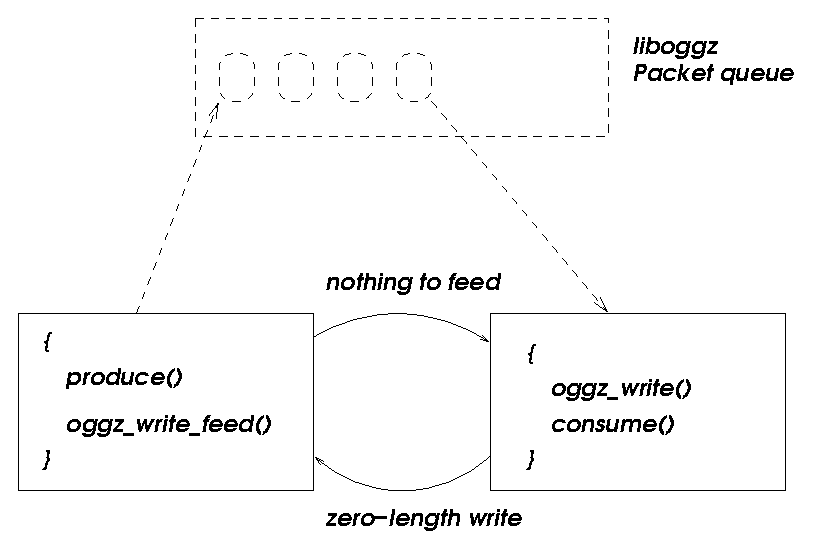
\includegraphics[width=10cm]{forcefeed}\caption{Force Feeding OGGZ}
\end{center}
\end{figure}


The following example code generates a stream of ten packets, each containing a single byte ('A', 'B', ... , 'J'):



\footnotesize\begin{verbatim}
#include <stdlib.h> /* exit */
#include <oggz/oggz.h>

static long serialno;
static ogg_int64_t granulepos = 0;
static ogg_int64_t packetno = 0;

int
main (int argc, char * argv[])
{
  char * progname, * filename = NULL;
  OGGZ * oggz;
  ogg_packet op;
  unsigned char buf[1];
  long n;

  progname = argv[0];
  if (argc > 1) filename = argv[1];

  if (filename) {
    oggz = oggz_open (filename, OGGZ_WRITE);
  } else {
    oggz = oggz_open_stdio (stdout, OGGZ_WRITE);
  }

  if (oggz == NULL) {
    fprintf (stderr, "%s: Error creating oggz\n", progname);
    exit (1);
  }

  serialno = oggz_serialno_new (oggz);

  for (packetno = 0; packetno < 10; packetno++) {

    /* Create a packet */

    buf[0] = 'A' + (int)packetno;

    op.packet = buf;
    op.bytes = 1;
    op.granulepos = granulepos;
    op.packetno = packetno;
    
    if (packetno == 0) op.b_o_s = 1;
    else op.b_o_s = 0;
    
    if (packetno == 9) op.e_o_s = 1;
    else op.e_o_s = 0;
    
    /* Feed it to the Oggz packet queue */

    oggz_write_feed (oggz, &op, serialno, OGGZ_FLUSH_AFTER, NULL);
    
    granulepos += 100;
    packetno++;

    /* Write bytes from packetized bitstream to the output file */

    while ((n = oggz_write (oggz, 32)) > 0);
  }

  oggz_close (oggz);

  exit (0);
}
\end{verbatim}
\normalsize
 

